\SECTION{Design and Implementation}\label{sec:design_imple}
The design and implementation of Linux-RTXG, which provides a framework for CPU and GPU coordinated scheduling based on the LKM, is described as follows.
In particular, the approach taken for GPU scheduling and its integration to CPU scheduling are explained.
Due to a space constraint, the detail of LKM-based CPU scheduling is referred to in the RESCH project~\cite{kato2009loadable, asberg2012exsched}.


\SUBSECTION{Linux-RTXG}
\begin{figure}[t]
\begin{center}
\ifthesis
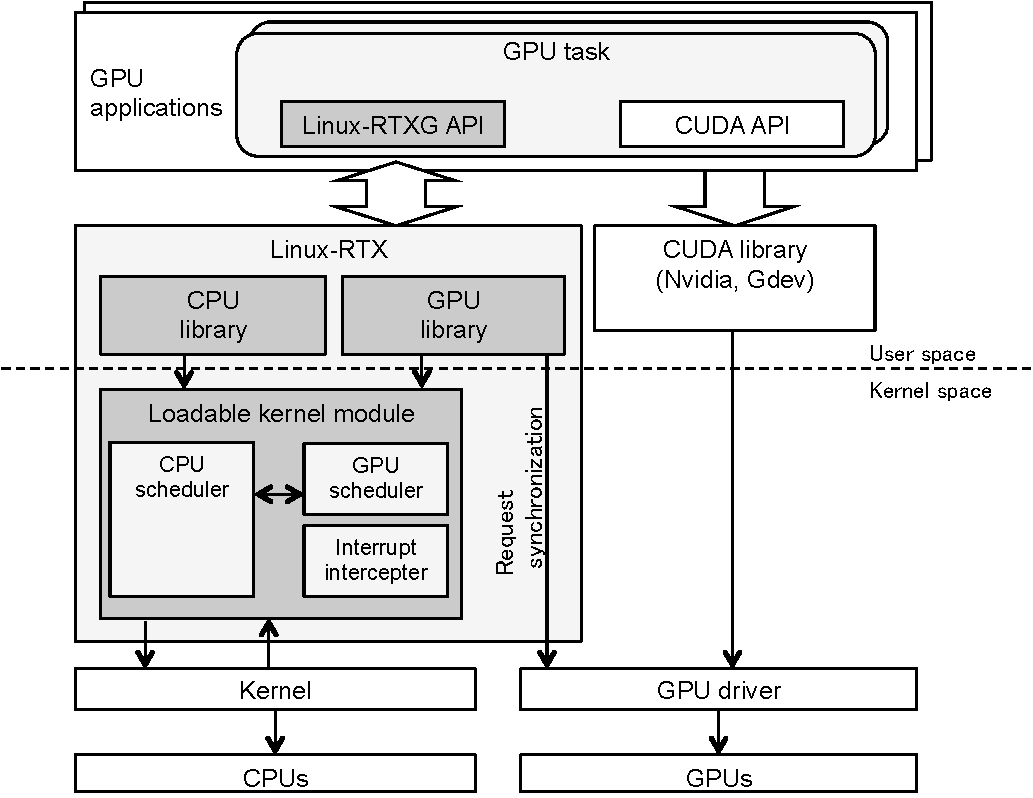
\includegraphics[width=0.8\textwidth]{img/overview.pdf}
%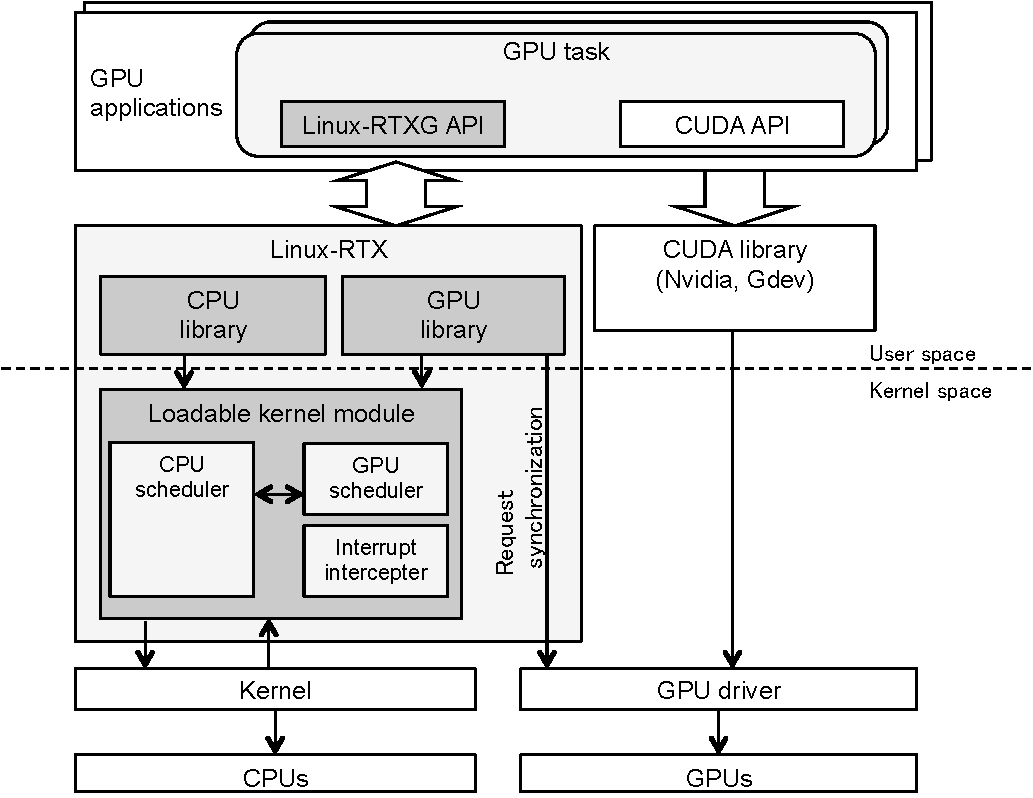
\includegraphics[width=1.0\textwidth]{img/overview.pdf}
\else
%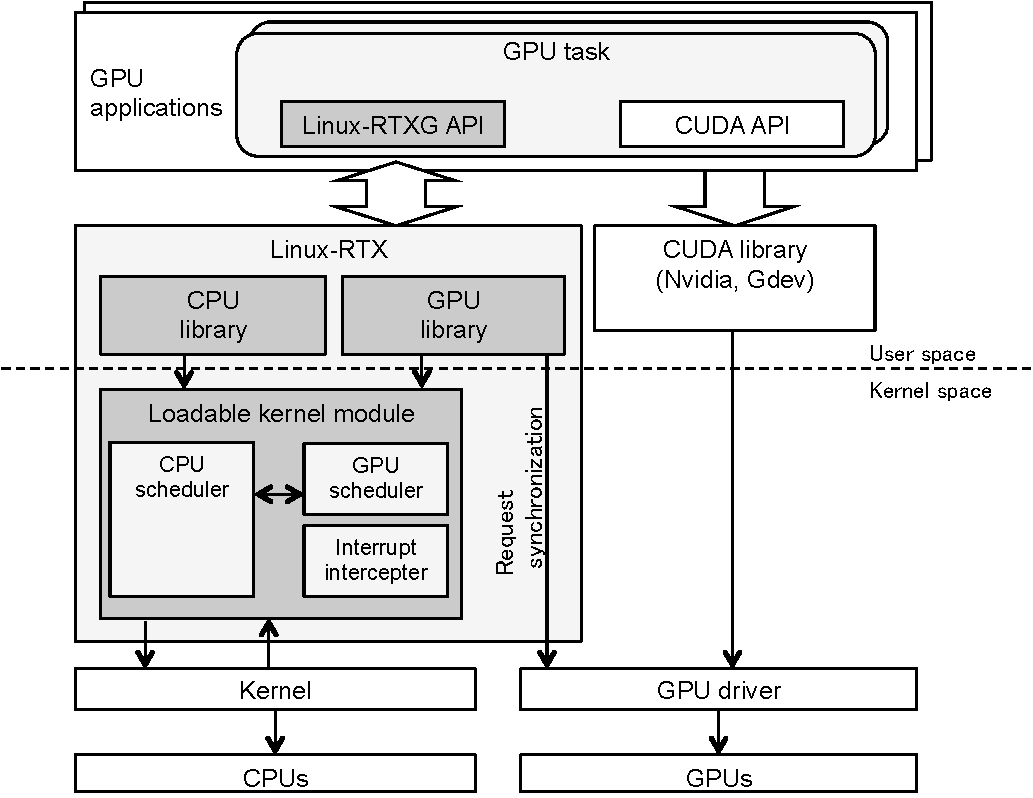
\includegraphics[width=0.35\textwidth]{img/overview.pdf}
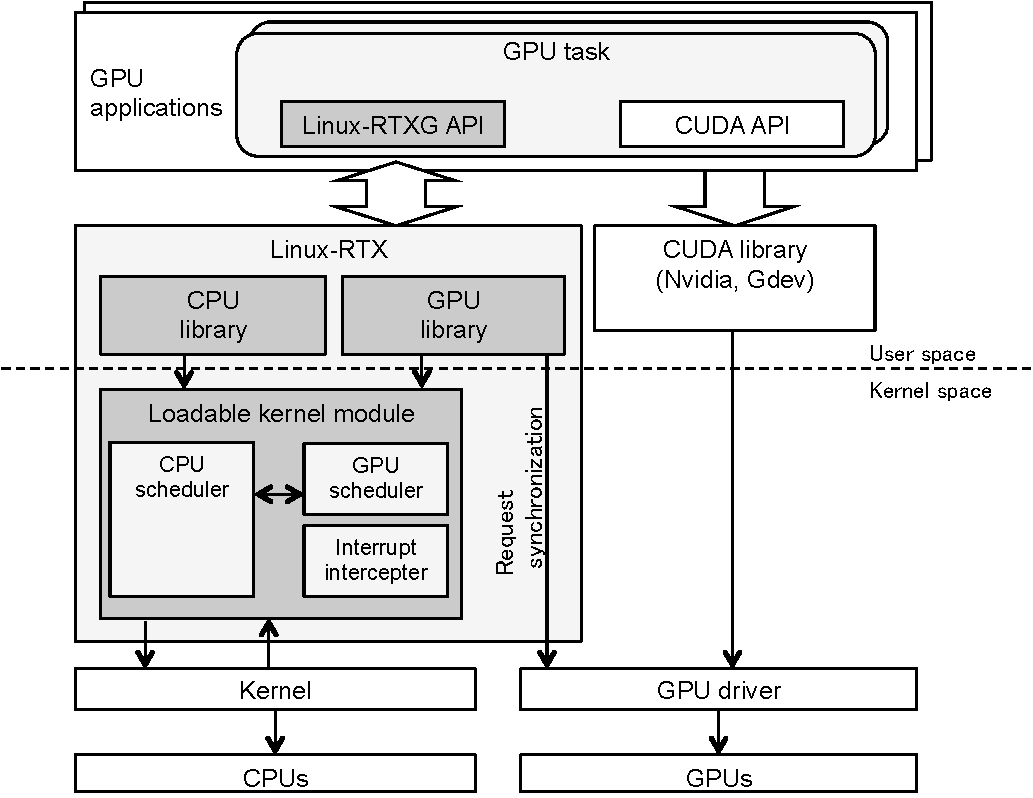
\includegraphics[width=0.47\textwidth]{img/overview.pdf}

\fi
\caption{Architectural overview of Linux-RTXG.}
\vspace{-4mm}
\label{fig:overview}
\end{center}
\end{figure}

An architectural overview of Linux-RTXG is shown in Figure~\ref{fig:overview}.
The system architecture of Linux-RTXG can be divided into two parts.
First, the Linux-RTXG core contains a CPU scheduler and a GPU scheduler with a resource-reservation mechanism.
The implementation of the Linux-RTXG core is provided in the kernel space by an LKM.
It can thus use exported Linux kernel functions, such as $schedule()$, $mod\_timer()$, $wake\_up\_process()$, and $set\_cpus\_allowed\_ptr()$.
These functions can be called from the user-space interface by using the input/output control (ioctl) system call, which is a standard system call for device drivers.
Secondly, the Linux-RTXG library provides an independent synchronization method for coordinated management of CPU and GPU resources.
The independent synchronization method can be used on top of a proprietary driver~\cite{nvidia:cuda_zone} as well as an open-source driver~\cite{nouveau}.
Note that this method is required to manage interrupts for GPU scheduling without modifying any codes of the OS kernel and device drivers.

\SUBSECTION{GPU Scheduling}
\begin{table*}[!t]
\begin{center}
\caption{A basic set of APIs for Linux-RTXG.}
\label{tab:rtx-api}
\ifthesis
\begin{tabular}{|l|p{25em}|} \hline
\else
\begin{tabular}{|l|p{53em}|} \hline
\fi
rtx\_gpu\_open() & Registers itself to Linux-RTXG and creates a scheduling entity. It must be called first. \\ \hline
rtx\_gpu\_device\_advice() & Obtains recommendations for which GPU devices to use. \\ \hline
rtx\_gpu\_launch() & Controls timing of launch of the GPU kernel , (i.e., a scheduling entry point). It must be called before the CUDA launch API. \\ \hline
rtx\_gpu\_sync() & Waits for the completion of execution of the GPU kernel by sleeping with TASK UNINTERRUPTIBLE status. \\ \hline
rtx\_gpu\_notify() & Sends a NOTIFY/FENCE command to the GPU. Either FENCE or NOTIFY is selected by a flag that is set by an argument.\\ \hline
rtx\_gpu\_close() & Releases the scheduling entity.\\ \hline
\end{tabular}
\end{center}
\vspace{-4mm}
\end{table*}

As well as being mostly based on the interrupt-driven method for GPU synchronization, Linux-RTXG is partly based on the API-driven method.
The scheduler is invoked only when computation requests are submitted.
The basic APIs supported by Linux-RTXG are listed in Table~\ref{tab:rtx-api}.
Note that some APIs have arguments and others do not.
Being independent of GPU runtimes, Linux-RTXG does not modify the existing CUDA API to cope with proprietary software.
However, CUDA application programs must add the Linux-RTXG APIs to use the functionality of Linux-RTXG.


The sample code including the Linux-RTXG APIs is shown in Figure~\ref{fig:sample}.
GPU tasks are provided with function calls to Linux-RTXG at strategic points.

\begin{figure}[!t]
\begin{center}
\begin{tabular}{l}
\hline\hline
{\scriptsize \verb|void gpu_task(){        |}\\
{\scriptsize \verb| /* variable initialization */ |}\\
{\scriptsize \verb| /* calling RESCH API */ |}\\
{\scriptsize \verb| dev_id = rtx_gpu_device_advice(dev_id); |}\\
{\scriptsize \verb| cuDeviceGet(&dev, dev_id); |}\\
{\scriptsize \verb| cuCtxCreate(&ctx, SYNC_FLAG, dev); |}\\
{\scriptsize \verb| rtx_gpu_open(&handle, vdev_id); |}\\
{\scriptsize \verb| /* Module load and set kernel function */ |}\\
{\scriptsize \verb| /* Device memory allocation */ |}\\
{\scriptsize \verb| /* Memory copy to device from host */ |}\\
{\scriptsize \verb| rtx_gpu_launch(&handle); |}\\
{\scriptsize \verb| cuLaunchGrid(function, grid_x, grid_y); |}\\
{\scriptsize \verb| rtx_gpu_notify(&handle); |}\\
{\scriptsize \verb| rtx_gpu_sync(&handle); |}\\
{\scriptsize \verb| /* Memory copy to host from device */ |}\\
{\scriptsize \verb| /* Release allocated memory */ |}\\
{\scriptsize \verb|}|}\\
\hline\hline
\end{tabular}
\caption{Sample code with the Linux-RTXG APIs.}
\vspace{-2mm}
\label{fig:sample}
\end{center}
\end{figure}

\begin{figure}[!t]
\begin{center}
 \ifthesis
 %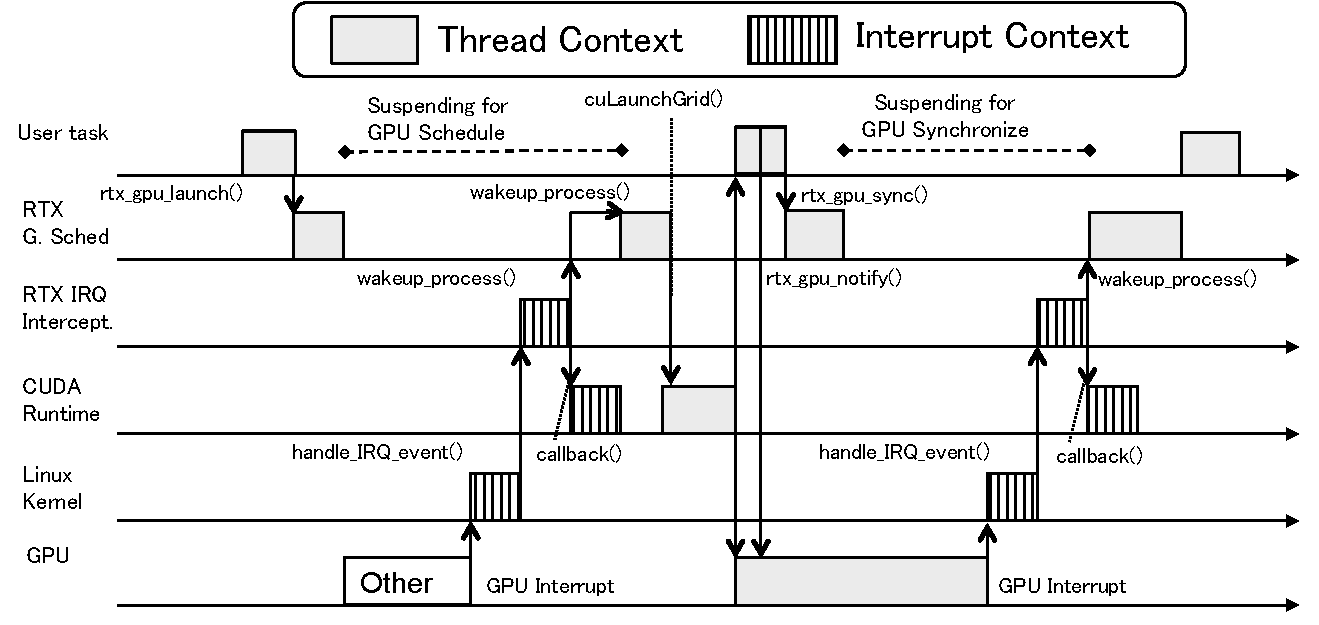
\includegraphics[width=\textwidth]{img/gsched_controlflow.pdf}
 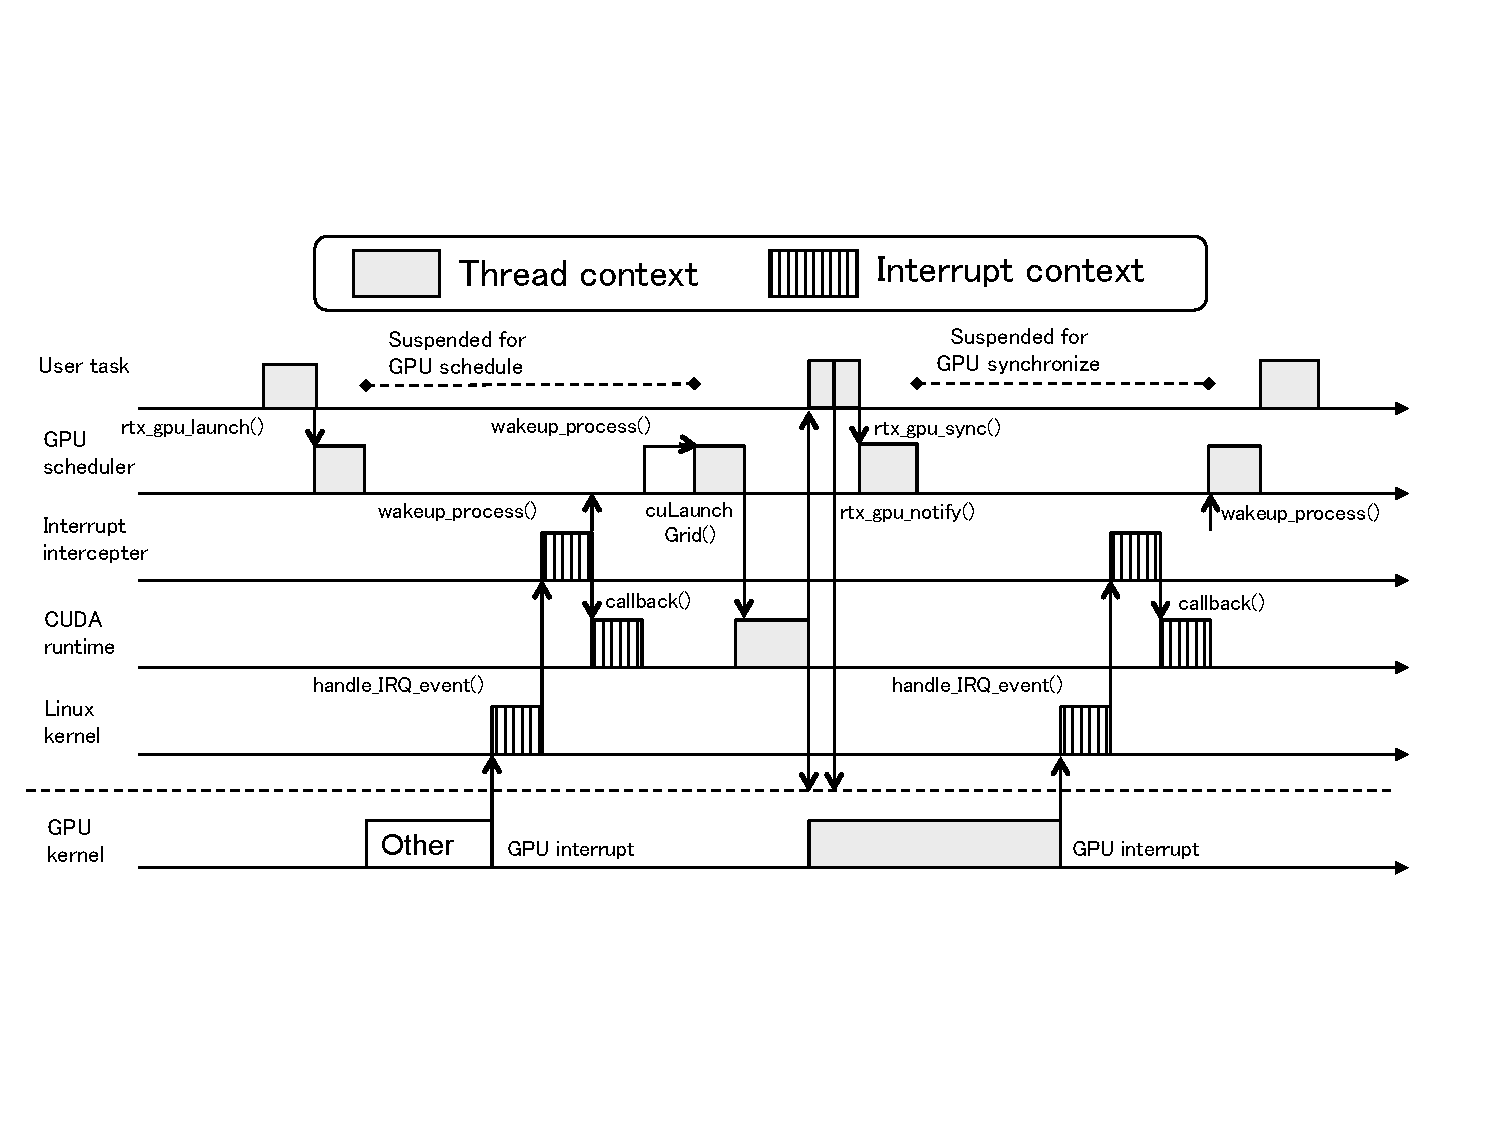
\includegraphics[width=\textwidth]{img/temp3.pdf}
 \else
% 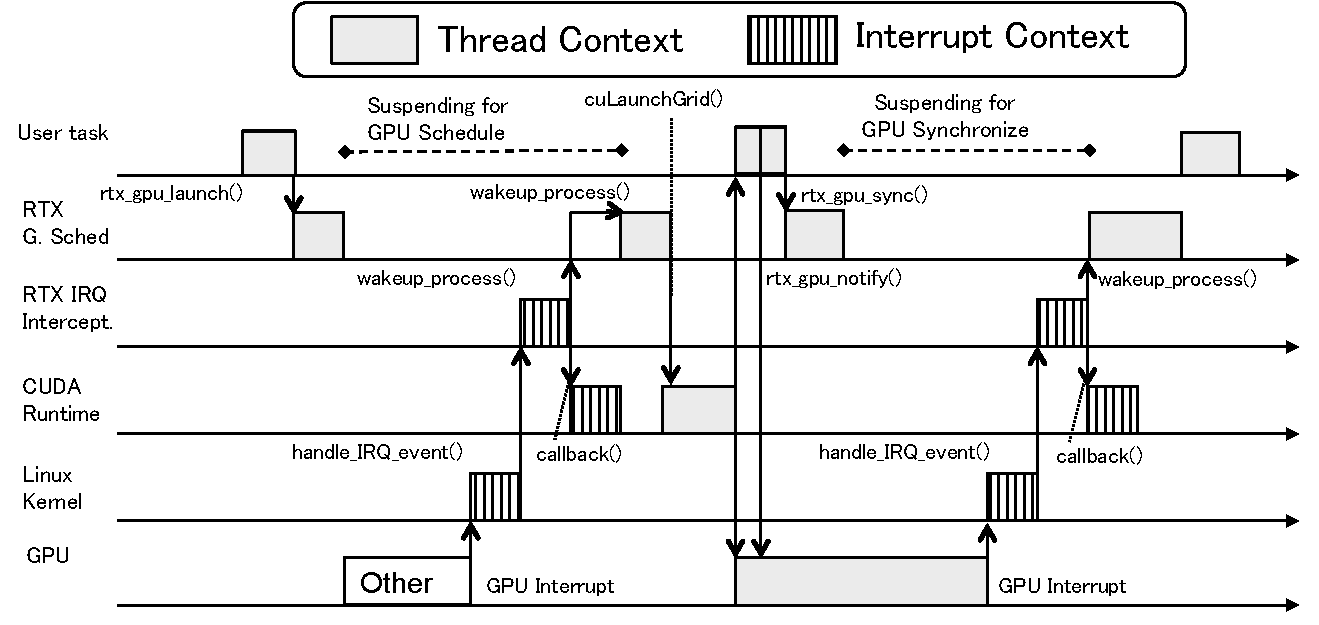
\includegraphics[width=0.5\textwidth]{img/gsched_controlflow.pdf}
 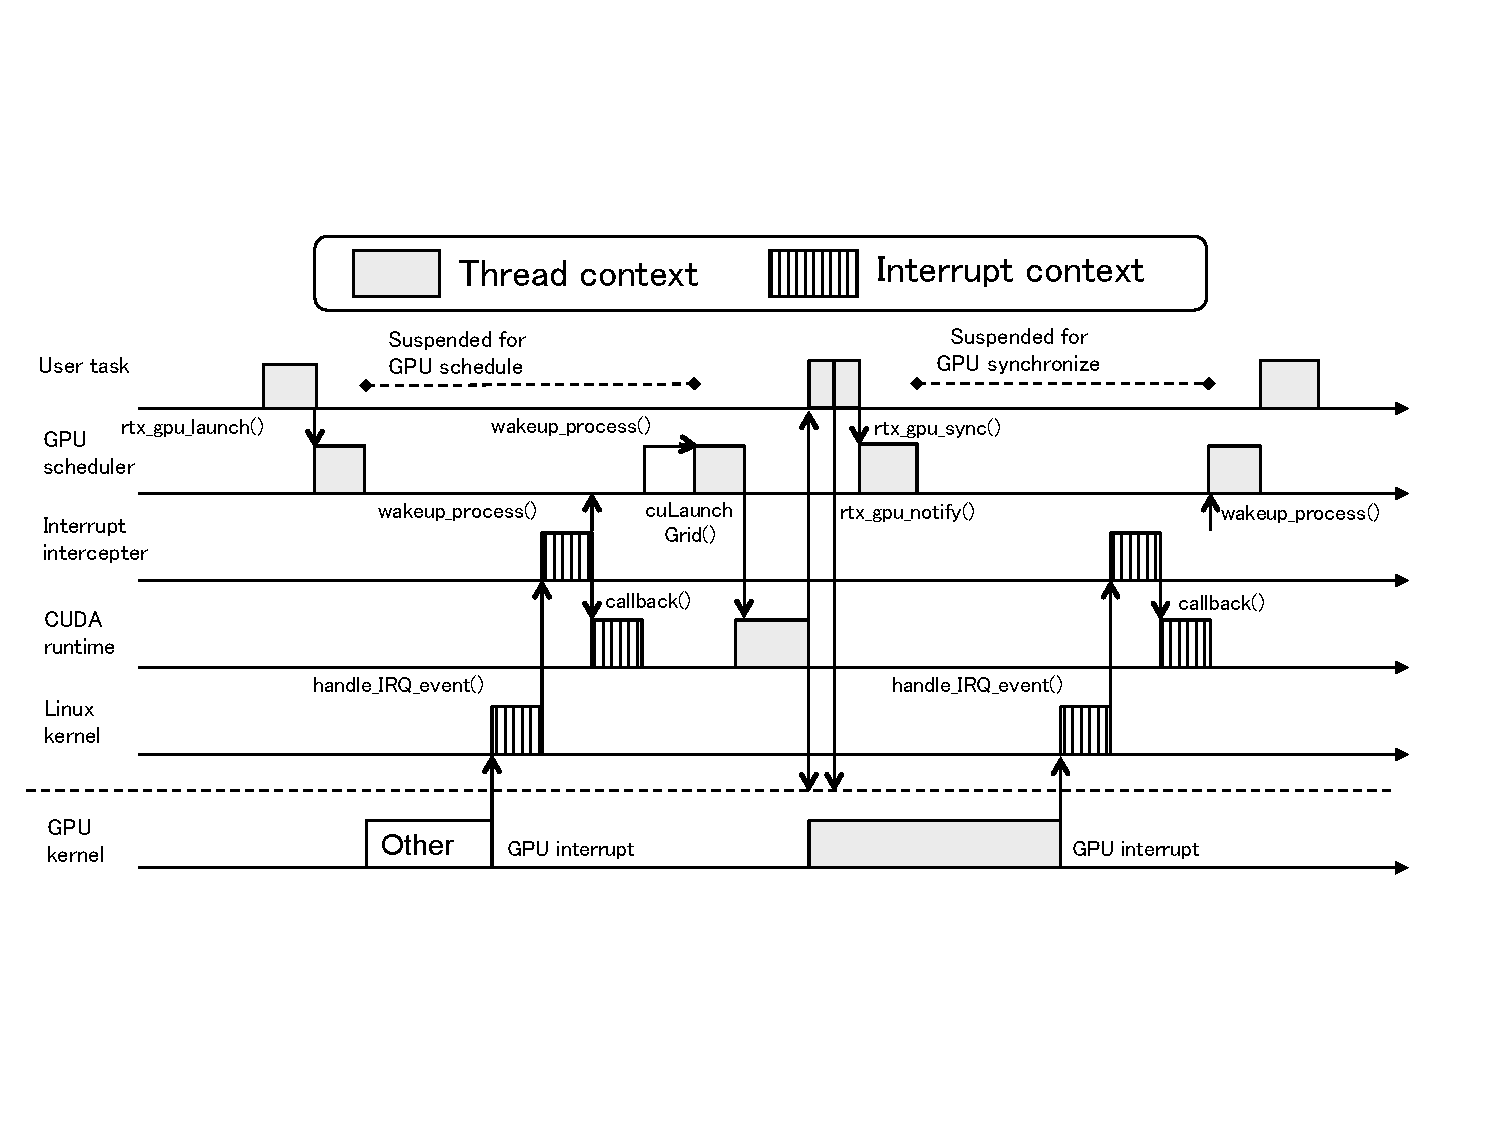
\includegraphics[width=0.5\textwidth]{img/temp3.pdf}
 \fi
\caption{Execution flow of a GPU task.}
\vspace{-4mm}
\label{fig:controlflow}
\end{center}
\end{figure}

The execution flow of the GPU task managed by the Linux-RTXG APIs is shown in Figure~\ref{fig:controlflow}.
Note that this example is restricted to a single GPU kernel.
The GPU task can control the timing that the GPU kernel is invoked by calling $rtx\_gpu\_launch()$.
After this function call, the task is suspended until it receives an interrupt so that other GPU kernels can be launched.
When execution of the GPU kernel is completed, an interrupt is raised by the GPU, and the corresponding interrupt handler is executed by the Linux kernel.
The interrupt interceptor awakens some suspended tasks according to the priority.
The awakened task proceeds to launch the GPU kernel by using a CUDA API, such as $cuLaunchGrid()$.
After the GPU kernel is launched, the task is going to register NOTIFY to set up an interrupt by $rtx\_gpu\_notify()$, and it is put into sleep mode again until it receives the interrupt by $rtx\_gpu\_sync()$.
Dispatching the subsequent task is performed by the GPU scheduler, which is called upon by the interrupt from the GPU.
Linux-RTXG manages the order of task execution according to this flow.


A hierarchical scheduling mechanism that applies the concept of virtual GPUs to combine specified GPU tasks by a group is presented in the following.
The virtual GPUs are created by a resource-reservation mechanism, while GPU scheduling uses a priority mechanism.
Specifically, each invocation of the GPU kernel is associated with a scheduling entity, and Linux-RTXG allocates the scheduling entities to virtual GPUs.
The virtual GPUs can belong to any physical GPUs.
In the case of Linux-RTXG, computing resources are distributed to virtual GPUs.

The pseudo-code of the Linux-RTXG scheduler is shown in Figure~\ref{fig:scheduling}.
This code works under the assumption that $on\_arrival$ is called when a GPU task requests to launch the GPU kernel.
When $on\_arrival$ is called, the GPU task checks whether the given execution permission is held by the allocated virtual GPU as well as the allocated scheduling entity.
If the virtual GPU to which the GPU task belongs does not hold the execution permission, the GPU task is enqueued to $wait\_queue$ and suspended.
Otherwise, the GPU task can launch the GPU kernel.
After a while, $on\_completion$ is called by the scheduler thread when the launched GPU kernel is completed, and the next set of a virtual GPU and a GPU task can be selected.
At the end of $on\_completion$, the selected GPU task is woken up.

\begin{figure}[!t]
\begin{center}
\begin{tabular}{l}
\hline
{\scriptsize \verb| se: Scheduling entity |}\\
{\scriptsize \verb| se->vgpu: Group that belongs to se|}\\
{\scriptsize \verb| se->task: Task that is associated with se |}\\
{\scriptsize \verb| vgpu->parent: Physical GPU identifier|}\\
\hline
{\scriptsize \verb|void on_arrival(se) {|}\\
{\scriptsize \verb| check_permit_vgpu(se->vgpu)    |}\\
{\scriptsize \verb| while(!check_permit_se(se)){|}\\
{\scriptsize \verb|   enqueue(se->vgpu,se); |}\\
{\scriptsize \verb|   sleep_task(se->task); |}\\
{\scriptsize \verb| }|}\\
{\scriptsize \verb|}|}\\
{\scriptsize \verb|void on_completion(se) {|}\\
{\scriptsize \verb| reset_the_permit(se->vgpu, se)|}\\
{\scriptsize \verb| n_vgpu = pick_up_the_next_vgpu(se->vgpu->parent) |}\\
{\scriptsize \verb| se = pick_up_the_next_se(n_vgpu)|}\\
{\scriptsize \verb| if(se) {|}\\
{\scriptsize \verb|   dequeue(se->vgpu,se);|}\\
{\scriptsize \verb|   wakeup_task(se->task);|}\\
{\scriptsize \verb| }|}\\
{\scriptsize \verb| set_the_permit(se->vgpu, se)|}\\
{\scriptsize \verb|}|}\\
\hline
\end{tabular}
\caption{High-level pseudo-code of the Linux-RTXG scheduler.}
\vspace{-8mm}
\label{fig:scheduling}
\end{center}
\end{figure}

\SUBSECTION{GPU Synchronization}
The independent-synchronization and interrupt-interception mechanisms are described next.
The independent-synchronization mechanism invokes NOTIFY and FENCE without using the GPU runtime API.
The interrupt-interception mechanism enables interrupt-driven invocation of the scheduler without modifying either the OS kernel or device drivers.
By this means, Linux-RTXG is not required to modify the OS kernel and device drivers, while being able to create the scheduling points for GPU tasks.

\textbf{Independent-synchronization Mechanism:} The independent-synchronization mechanism using NOTIFY and FENCE is described as follows.
This mechanism invokes an interrupt using NOTIFY, and writes the fence value using the GPU microcontrollers and FENCE.
NVIDIA's proprietary software uses the ioctl interface to communicate with the kernel space and the user space.
These ioctl interfaces provide driver functions, such as device-memory allocation, obtaining GPU states and memory mapping.
Gdev provides a runtime library that can control the GPU on top of NVIDIA's proprietary driver by using these ioctl interfaces.
The mechanism also uses an ioctl interface similar to Gdev in order to send commands to the GPU.
Specifically, the mechanism is divided into two processes: (i) initialization and (ii) notification.

The initialization process generates a dedicated GPU context.
This process creates a virtual address space, allocates an indirect buffer object for commands, and creates a context object that is required to employ the FIFO engine, followed by allocation of a kernel-memory object and mapping of the FIFO-engine registers to host memory space through a memory-mapped I/O (MMIO).
The FIFO engine is a GPU microcontroller that decodes and dispatches the commands sent from the host CPU side.

The notification process sends commands to a GPU compute engine or a GPU data-copy engine by the $iowrite$ function associated with the mapped FIFO-engine registers so that an interrupt will be raised from the GPU to the CPU.
The compute engine and the data-copy engine are such GPU microcontrollers that control the states of GPU computation and data transfer.
They are also used to switch GPU contexts on the GPU computation and data transfer.
Note that this independent-synchronization mechanism requires the information of ioctl interfaces.
Therefore, it depends on the GPU architecture and implementation of device drivers.

\textbf{Interrupt Interception:} Interrupts are handled by the ISR that is registered to the Linux kernel by the device driver.
The scheduler function is required to receive the interrupts and identify them by reading the GPU status register.
The GPU status register must be read by the OS scheduler before it is reset by the ISR.

The Linux kernel has a structure that holds interrupt parameters, called $irq\_desc$, for each interrupt number.
This structure has an internal sub-structure called $irq\_action$, which includes the ISR callback pointer.
The $irq\_desc$ structure is allocated to the global kernel memory space, and is freely accessible from the kernel space.
Therefore, not only the Linux kernel but also external LKMs can obtain the information of $irq\_desc$ and the ISR callback pointer.
The ISR callback pointer associated with the GPU device driver is obtained, and a new interrupt interception ISR is registered in the Linux kernel.
Finally, interrupts from the GPU through the ISR can be intercepted, and the callback pointer can be retained.
In addition, I/O registers are mapped from the PCIe base address registers (BAR) to the kernel memory space by the device driver ~\cite{fujii:icpads2013,kato2013zero}.
Therefore, Linux-RTXG remaps the BAR0 to the allocated space by using $ioremap()$ when the ISR is initialized.
The interrupt-interception mechanism can identify the source of every interrupt by reading this remapped space.


\SUBSECTION{Scheduler Integration}
The mainline Linux scheduler implements the following three real-time scheduling policies:
\begin{itemize}
\item $SCHED\_DEADLINE$
\item $SCHED\_FIFO$
\item $SCHED\_RR$
\end{itemize}

$SCHED\_DEADLINE$ is the implementation of CBS and EDF, which is the latest real-time scheduler for Linux introduced in version 3.
14.0, while $SCHED\_FIFO$ and $SCHED\_RR$ represent fixed-priority scheduling.
Unfortunately, synchronization does not work with the SCHED\_DEADLINE scheduling policy for GPU tasks.
Two problems concerning implementation must therefore be solved.
The first problem is attributed to the implementation of $sched\_yield()$.
Note that $sched\_yield()$ uses $yield()$ in the kernel space.
Releasing the CPU by $sched\_yield()$ while waiting for I/O in polling makes it possible to utilize CPU time more efficiently.
However, $sched\_yield()$ will set the remaining execution time of the polling task to zero by treating it as a parameter of $SCHED\_DEADLINE$.
As a result, the task cannot be executed until the runtime is replenished in the next period.
This means that $sched\_yield()$ should not be called while polling in $SCHED\_DEADLINE$.
However, $sched\_yield()$ is frequently used by device drivers and libraries.
Real-time performance of GPU computing, even in CUDA, could be affected by this problem.
This problem is addressed by limiting the GPU synchronization method to NOTIFY, namely, eliminating the potential of FENCE, in the $SCHED\_DEADLINE$ scheduling policy.

The second problem is subject to the implementation of wake-up and sleep functions, particularly the check equation~\eqref{eq} when restoring a task from the sleep state.
If equation ~\eqref{eq} holds, the runtime is replenished, and the absolute deadline is set to the next cycle deadline.

{\scriptsize
\begin{equation}
\frac{Absolute\_Deadline - Current\_Time}{Remaining\_Runtime} > \frac{Relative\_Deadline}{Period} \label{eq}
\end{equation}
}

This check condition is revised so that the GPU execution time is subtracted from $Remaining Runtime$ when a task is restored by the GPU kernel execution, except when a task is restored by the period.
